\section{Typical designs of Tangible User Interfaces}

In this section we will discuss different hardware implementations of tangible user interfaces and take a look on the different design spaces they are used in. 
% The interpretation of tangible user interfaces varies throughout the field. Ullmer and Ishii \cite{ullmer97} 

Design spaces that we discuss in this paper include but are not limited to
\begin{itemize}
\item  Information Visualization
\item Architectural Contexts
\item Geographical Contexts
\item Entertainment
\end{itemize}

Shaer and Hornecker \cite{hornecker10} also give the following list of possible application domains:
\begin{itemize}
\item TUIs for Learning
\item Problem Solving and Planning
\item Information Visualization
\item Tangible Programming
\item Entertainment, Play, and Edutainment
\item Music and Performance
\item Social Communication 
\item Tangible Reminders and Tags
\end{itemize}

For the hardware description we will retain at two implementations: the metaDESK system by Ullmer and Ishii \cite{ullmer97} and Tangible Views by Spindler, Tominski, Schuhmann and Dachselt \cite{spindler10}
The metaDESK system hereby depicts a system whose components are fixed and attached to the system, whereas in the Tangible Views system the views are simple physical surfaces with no restrictions on size and shape. 

The last part of this section is a view on social aspects of Tangible User Interfaces.

\subsection{metaDESK}
One of the attemps in broadening the input possibilities to different devices is the metaDESK system introduced by Ullmer and Ishii \cite{ullmer97}. They describe a "Tangible User Interface" (TUI) as a user interface employing physical objects, instruments, surfaces, and spaces as physical interfaces to digital information. The metaDESK system consists of: a desk, a nearly-horizontal backprojected graphical surface; an active lens an arm-mounted flat-panel display; one or more passive lenses, an optically transparent surface through with the desk projects; and an assortment of physical objects an instruments which are used on the desk's surface. The components are sensed by an array of optical, mechanical and electromagnetic field sensors. An image of such a setup can be seen in Figure \ref{fig:metadesk} an an outline of the hardware positioning in Figure \ref{fig:metadeskhardware}.

%http://www.guillaumeriviere.name/collection/tabletop.html
\begin{figure}
\centering
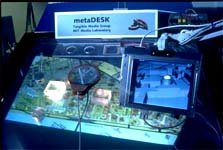
\includegraphics[width=0.45\textwidth]{figures/metaDesk.jpg}
\caption{metaDESK}
\label{fig:metadesk}
\end{figure}

%http://www.guillaumeriviere.name/collection/tabletop.html
\begin{figure}
\centering
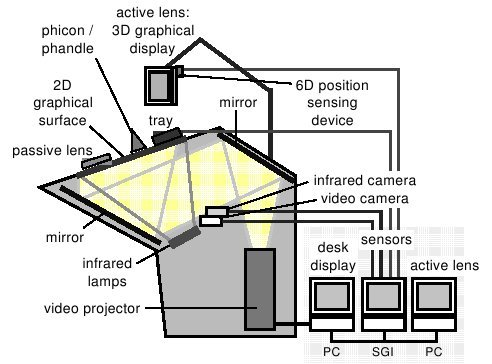
\includegraphics[width=0.45\textwidth]{figures/metaDeskHardware.jpg}
\caption{metaDESK Hardware Overview}
\label{fig:metadeskhardware}
\end{figure}

The focus lies on the use of real physical objects as driving elements of human-computer interaction. The approach of Ullmer and Ishii allthough tries to take elements of the GUI and bringing it into the real world as well as pushing forward from the unaugmented physical world, inheriting from vaious historical instruments and devices often "obsoleted" by the advent of the computer, like the active lens which is based on a jeweler's magnifying lens. The models for the objects are taken from everyday objects from home, scientific instruments or drawing and design tools. The material they used was transparent machined acrylic, designed to minimize occlusion of the desk surface.

The GUI icons are instantiated as "phicons" (physical icons), menus and handles are instantiated as TUI "trays" and "phandles" (physical handles), scales and scrollbars as TUI instruments such as a rotation constraint instrument. 

To test the system they implemented a prototype application called "Tangible Geospace" allowing interaction with geographical space.
The models themselves act as information containers about the object they represent as well as physical handles for manipulating the map.

The arm mounted active lens is coupled to the models and displays three-dimensional views of the scene and moving the lens makes it possible to navigate throu 3D space. This allows a seamless interaction with three spaces at once: the physical space of the object, the 2D graphical space of the desk's surface and the 3D graphical space of the active lens.

It is also possible to place a second object on the table, allowing the user to scale or rotate the map by moving the objects with respect to each other. This also allows collaboration as each object may be manipulated by an individual user. The sensing is performed by a computer-vision system inside the desk unit, along with magnetic -field position sensors and electrical contact sensors.

The passive lenses consist of a transparent surface that functions as an independent display when augmented by the back-projected desk. Since they are passive transparent surfaces, many vaiously afforded lenses might be used simultaneously with no additional active display resources.

As alternative to the two phicon scaling/rotation interaction, a rotation constraint instrument made of two cylinders mechanically coupled by a sliding bar might be used.
Albeit the extension of input methods it is not the goal of metaDESK to replace GUIs, but rather to complement them by providing new opportunities for human-computer interaction. 



\subsection{Tangible Views}
Spindler, Tominski, Schuhmann and Dachselt \cite{spindler10} introduce 'tangible views' for use in Information Visualization as spatially aware lightweight displays that can be interacted with by moving them through the physical space on or above a tabletop surface. 

The motivation for their project is the difficulty of encoding all information in a single image once a data set exceeds a certain size or complexity. This problem can be solved spatially by providing multiple views on the data or embedding additional local views in the visualization or it can be solved temporally by changing the representations over time. They define a tangible view as a physical surface, that users can hold in their hands with no restrictions on size and shape.
 
Tangible views serve two purposes: It is used as a local display in conjunction with a tabletop display, and as an input device. The specific graphical information is projected onto the tangible view and three dimensional manipulation of a tangible view is tracked in space to make six degrees of freedom available: position (x, y, z) with respect to the interaction space and local orientation of the tangible view ($\alpha$, $\beta$, $\gamma$). It is also possible to use multiple tangible views at the same time. 

In summary tangible views:
\begin{itemize}
\item Integrate display an interaction device.
\item Enhance common 2D interaction with additional 3D interaction
\item Replace virtual views by physical, tangible views.
\end{itemize}

Tangible views do not exist on their own, but are integrated into an environment of one or more stationary displays of arbitrary size, shape and orientation. 
They also describe a basic display configuration consisting of a horizontal tabletop for the main context view and tangible views as local views into the information space. This relates to the focus and context concept.

As Tangible Views play an important role in Information Visualization we will treat this subject in section four in more detail.


\subsection{Including social aspects}
Hornecker and Buur \cite{hornecker06} extend the thought of tangible user interfaces further to 'tangible interactions'. They introduce a framework that focuses on the interweaving of the material/physical and the social, laying the ground for collaboration-sensitive tangible interaction design. It relies on tangibility and full-body interaction and gives computational resources and data material form, embedding computing in the everyday environment, digitally augmenting physical space and supporting intuitive use. 

Designing tangible interfaces requires not only designing the digital but also the physical, and their interrelationships within hybrid ensembles, as well as designing new types of interaction that can be characterized as full-body, haptic, and spatial.
Applications previously not considered interfaces are turning into such and computing is increasingly embedded in physical environments.

They distinguished three different views on tangible interfaces:
\begin{itemize}
\item Data-centered view: Here 'tangible interfaces' are understood as utilizing physical representation and manipulation of digital data, offering interactive couplings of ohysical artifacts with "computationally mediated digital information", Eg. Ullmer and Ishii
\item Expressive-Movement-centered view: Aiming to design interaction itself by emphasizing bodily interaction with objects, exploiting the "sensory richness and action potential of physical objects" so that "meaning is created in the interaction". <--!!quote!!
\item Space-centered view: 'Interactive spaces' as "Interactive systems, physically embedded within real spaces, offer opportunities for interacting with tangible devices" and so "trigger display of digital content or reactive behaviours" The body is used as interaction device and display.
\end{itemize}

Tangible interaction encompasses a broad range of systems and interfaces, building upon and synthesizing these views. These share the following characterisitcs: tangibility and materiality, physical embodiment of data, embodied interaction and bodily movement as an essential part of interaction, and embeddednes in real space, designing the interaction itself and exploiting the richness of bodily movement.

Their framework is structured around four interrelated themes:
\begin{itemize}
\item Tangible Manipulation:  material representations with distinct tactile qualities which are physically manipulated.
\item Spatial Interaction: tangible interaction is embedded in real space and therefore occurs by movement in space.
\item Embodied Facilitation: how the configuration of material objects and space affects and directs group behaviour.
\item Expressive Representation: material and digital representations employed ba tangible interaction systems, their expressiveness and legibility.
\end{itemize}

\begin{figure}
\centering
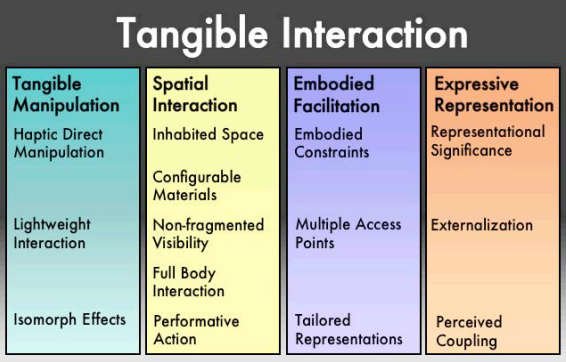
\includegraphics[width=0.45\textwidth]{figures/tangibleInteraction.png}
\caption{Tangible Interaction}
\label{fig:tangibleInteraction}
\end{figure}

Figure \ref{fig:tangibleInteraction} shows the design spaces of tangible interaction from specific on the left to the more general on the right. 

% Design and Hardware